\documentclass{article}
\usepackage{dingbat}
\usepackage[mathscr]{euscript}
\usepackage[
backend=biber,
style=alphabetic,
sorting=ynt
]{biblatex}
\addbibresource{bibliography.bib}

 \usepackage{graphicx}
\graphicspath{ {./images/} }


\title{Experiment Protocol}
\author{Will Thompson}

\begin{document}

\maketitle

% --------------------------------------------------------------------
\section{Introduction}

Entity linking is the task of assigning unique entity identifiers to mentions of entities in text \cite{sevgili_neural_2022}. There are two core data sources for this task: (1) a collection of unstructured documents $\mathscr{D}$ that contain a set $\mathscr{M}$ of text spans interpreted as entity mentions, and (2) a structured domain knowledge base $\mathscr{K}$ that contains a set $\mathscr{E}$ of uniquely identified entities, which can be anything of interest. Entity linking is the task of defining a function $\Gamma: \mathscr{M}X\mathscr{D} \rightarrow \mathscr{E}$ that maps a mention $m_{i} \in \mathscr{M}$ in document $d_{j} \in \mathscr{D}$ to a unique entity $e_{k} \in \mathscr{E}$.

My core research interest is in applying entity linking to \emph{clinical notes}, unstructured text that can be found in large quantities in electronic health records (EHR). There is a lot of potentially useful information in such notes, ranging from disease mentions, descriptions of symptoms, past medical history, response to treatments, and so on. While EHR also have large quantities of structured information, it turns out that the structured information that is available often provides an incomplete (or even  misleading) picture of a patient's clinical status. Notes in the EHR typically contain a more direct assessment of a patient's condition, and can be the sole source of information for areas such as medical symptoms, treatment response, cancer grading, and past medical history. There is a huge amount of information locked up in clinical notes, and clinical entity linking has many potentially use cases for research into diseases, measuring population health, creation of disease-specific registries, and clinical trial recruitment.

My general NLP-related research goal is to improve on the state of the art for clinical entity linking -- linking mentions of diseases, symptoms, treatments (etc.) in clinical notes to entity identifiers in domain knowledge bases such as the Unified Medical Language System (UMLS; \cite{bodenreider_unified_2004}), a large domain knowledge base created by the National Library of Medicine containing over 4 million clinically relevant entities linked into a semantic network. There are two highly salient background facts relevant to clinical entity linking. First, there is a general lack of labeled data. Due to privacy concerns and regulations (such as HIPAA), there are few publicly available corpora, and even fewer that are annotated with gold standard labels. Second, there is an abundance of knowledge bases such as the UMLS.

These two facts lead me to focus on \emph{self supervised} \cite{krishnan_self-supervised_2022} approaches to entity linking. These are approaches that leverage domain knowledge bases (such as the UMLS) to automatically generate candidate entity mentions to train entity linking models. Self-supervision has been successfuly used to overcome the general lack of annotated resources for the clinical domain. In particular for this paper, I will focus on the recent model \texttt{KRISSBERT}, proposed by \cite{zhang_knowledge-rich_2022}. This model has achieved state of the art for self-supervised approaches to biomedical entity linking. This will be the reference approach and baseline model for the research ideas proposed in this paper.


% --------------------------------------------------------------------
\section{Hypotheses}

My hypotheses are stated relative to a self-supervised approach to entity linking, with the following core assumptions:

\begin{itemize}
  \item \textbf{Assumption 1}: There are two data sources consisting of a collection of unlabeled text and a list of structured entities, which each have a unique identifer and a canonical name.
  \item \textbf{Assumption 2}: Self-supervised learning uses the entity names to generate entity mentions for training.

  \vspace{1em}
  For the purposes of this paper, I will make the following additional assumptions:

  \item  \textbf{Assumption 3}: There are multiple target domains $\mathscr{K}^{(i)}$, subsets of $\mathscr{K}$. Each target domain $\mathscr{K}^{(i)}$ contains a set of entities $\mathscr{E}^{(i)}$ that are subsets of $\mathscr{E}$. For example, if we use the UMLS as our knowledge base, there are subsets that describe cancer diseases, or heart disease, etc. Each of these target domains may also be affiliated with a specific collection of documents $\mathscr{D}^{(j)}$ subset of $\mathscr{D}$. For example, we may be interested in extracting cancer concepts from pathology notes, which have a much different structure and content than patient discharge notes.

  \item \textbf{Assumption 4}: The domain $\mathscr{E}^{(i)}$ may or may not have an annotated gold standard available for model training and testing. Where available, they can potentially be used to improve results derived solely from self-supervised models.
\end{itemize}

Given these assumptions, the following hypotheses relate to ways in which self-supervised entity linking models can be augmented and potentially improved:

\begin{itemize}
  \item \textbf{Hypothesis 1}: Relative to Assumptions (1-2), entity linking accuracy can be increased by generating higher-quality entity mention examples for training. \cite{zhang_knowledge-rich_2022} use exact string matching from texts to canonical entity names in the UMLS to generate training examples. They spot-checked a random sample and determined that this method achieved approximately 85\% accuracy (given the context, I'm assuming this means 0.85 \emph{precision} for linked entities from the generated mentions). Although this is quite good, and given the sheer volume of data they generate it performs well in practice, my hypothesis is we could do better by placing further restrictions on string matching -- such as requiring a minimum token length to reduce potential linguistic ambiguities. Reducing training noise will (hopefully) result in better model performance.

  \item \textbf{Hypothesis 2}: Relative to Assumptions (1-3), entity linking accuracy can be increased by using a domain-specific target corpus for pre-training or fine-tuning. \cite{zhang_knowledge-rich_2022} use PubMedBERT \cite{gu_domain-specific_2022}, trained on large amounts of PubMed abstracts. This is naturally a good corpus to use for the target domain of biomedical literature, but it might not be the best data source for clinical notes, which are drastically different in terms of content and structure. There are pre-existing language models trained on clinical notes (such as ClinicalBERT \cite{huang_clinicalbert_2020}) which may serve as a better foundation, and we can experiment with using very specific subsets of notes (such as pathology or radiology notes) to fine-tune to specific target domains.

  \item \textbf{Hypothesis 3}: At inference time, it appears to be common practice (e.g., \cite{zhang_knowledge-rich_2022}, \cite{jose_medlinker_2020}, \cite{logeswaran_zero-shot_2019}, \cite{wu_scalable_2020}) to use a nearest neighbour approach to select the top-K entities that are potentially best matches to a given entity mention. Relative to Assumptions (1-3), entity linking accuracy can be improved for specific target domains by pre-pruning the entity space for target-specific concepts, before performing nearest neighbour search. This seems like it couldn't possibly hurt (assuming we only care about the target concepts for a particular use case), and would very likely improve entity linking performance by removing irrelevant distractors.

  \item \textbf{Hypothesis 4}: Relative to Assumptions (1-4), entity linking accuracy can be increased by using labeled examples for a target domain to fine-tune the self-supervised model. This again seems like it couldn't possibly hurt, and the question is to what degree it might improve accuracy.

  % \item The nearest neighbour approach to inference can be improved by averaging the target entity representations, and then comparing entity mentions to these averaged representations.

  %\item Improve the re-ranking algorithm (\cite{zhang_knowledge-rich_2022}, Figure 2)
\end{itemize}

% The self-supervised entity linking model described in \cite{zhang_knowledge-rich_2022} completely side-steps the question of how to generate mentions at test/inference time. Training mentions are generated using exact string matching with unambiguous canonical entity names.
%
% \begin{enumerate}
%   \item In order to achieve good recall, mention generation should be approximate and relatively loose. We can use approximate string matching techniques
%   \item In order to avoid large numbers of false positives, we can develop a \emph{Nil} entity model.
% \end{enumerate}


% --------------------------------------------------------------------
\section{Datasets}

I will use the following datasets, each of which I have already accessed:

\begin{enumerate}
  \item UMLS \cite{bodenreider_unified_2004}: a large domain knowledge base created by the National Library of Medicine containing over 4 million clinically relevant entities linked into a semantic network.
  \item MedMentions \cite{mohan_medmentions_2019}: the largest available dataset mapping text to UMLS concepts. The texts consist of over 4,000 PubMed abstracts containing over 350,000 linked mentions. This dataset is widely used in the literature on biomedical entity linking.
  \item MIMIC-III \cite{goldberger_physiobank_2000}: a large database of deidentified health-related data associated with over 40,000 patients who stayed in critical care units of the Beth Israel Deaconess Medical Center between 2001 and 2012. The database includes a clinical notes table with over 2 million rows.
  \item Shared Annotated Resources (ShARe) SemEval 2015 corpus \cite{savova_guergana_analysis_nodate}, \cite{pradhan_semeval-2014_2014}: 531 deidentified clinical discharge summaries and radiology reports from the MIMIC clinical database. The ShARe corpus contains gold-standard annotations of disorder mentions and a set of attributes.
  \item RadGraph \cite{jain_saahil_radgraph_nodate}: a dataset of entities and relations in full-text radiology reports extracted from MIMIC chest x-rays. RadGraph contains a test set of 500 annotated notes, and a test set of 100 notes. Mention types fall under the two broad categories of Observation and Anatomy.
  % \item Phenotype annotations for patient notes in the MIMIC-III dataset (\cite{moseley_edward_phenotype_nodate}, \cite{gehrmann_comparing_2018}):
\end{enumerate}


% --------------------------------------------------------------------
\section{Metrics}

I will use two quantitative metrics:

\begin{enumerate}
  \item Top-K accuracy: this metric computes the number of times where the correct entity label is among the top k labels predicted. Top-1 accuracy will be my primary metric for evaluating systems.
  \item Mean reciprocal rank (MRR): MRR measures how far down the ranking the correct entity is. This will give a sense of ``how far off'' (on average) the true results are from being correctly predicted.
\end{enumerate}

In addition to using these quantitative metrics, I will be doing a qualitative error analysis to get a better sense of what is going on with the entity linking systems. I believe it will be particularly instructive to look at entities with ambiguous entity mentions (names that are shared across entity types). I will also be doing an ablation analysis to look at the specific contributions of the various components.

% --------------------------------------------------------------------
\section{Models}

\begin{figure}
  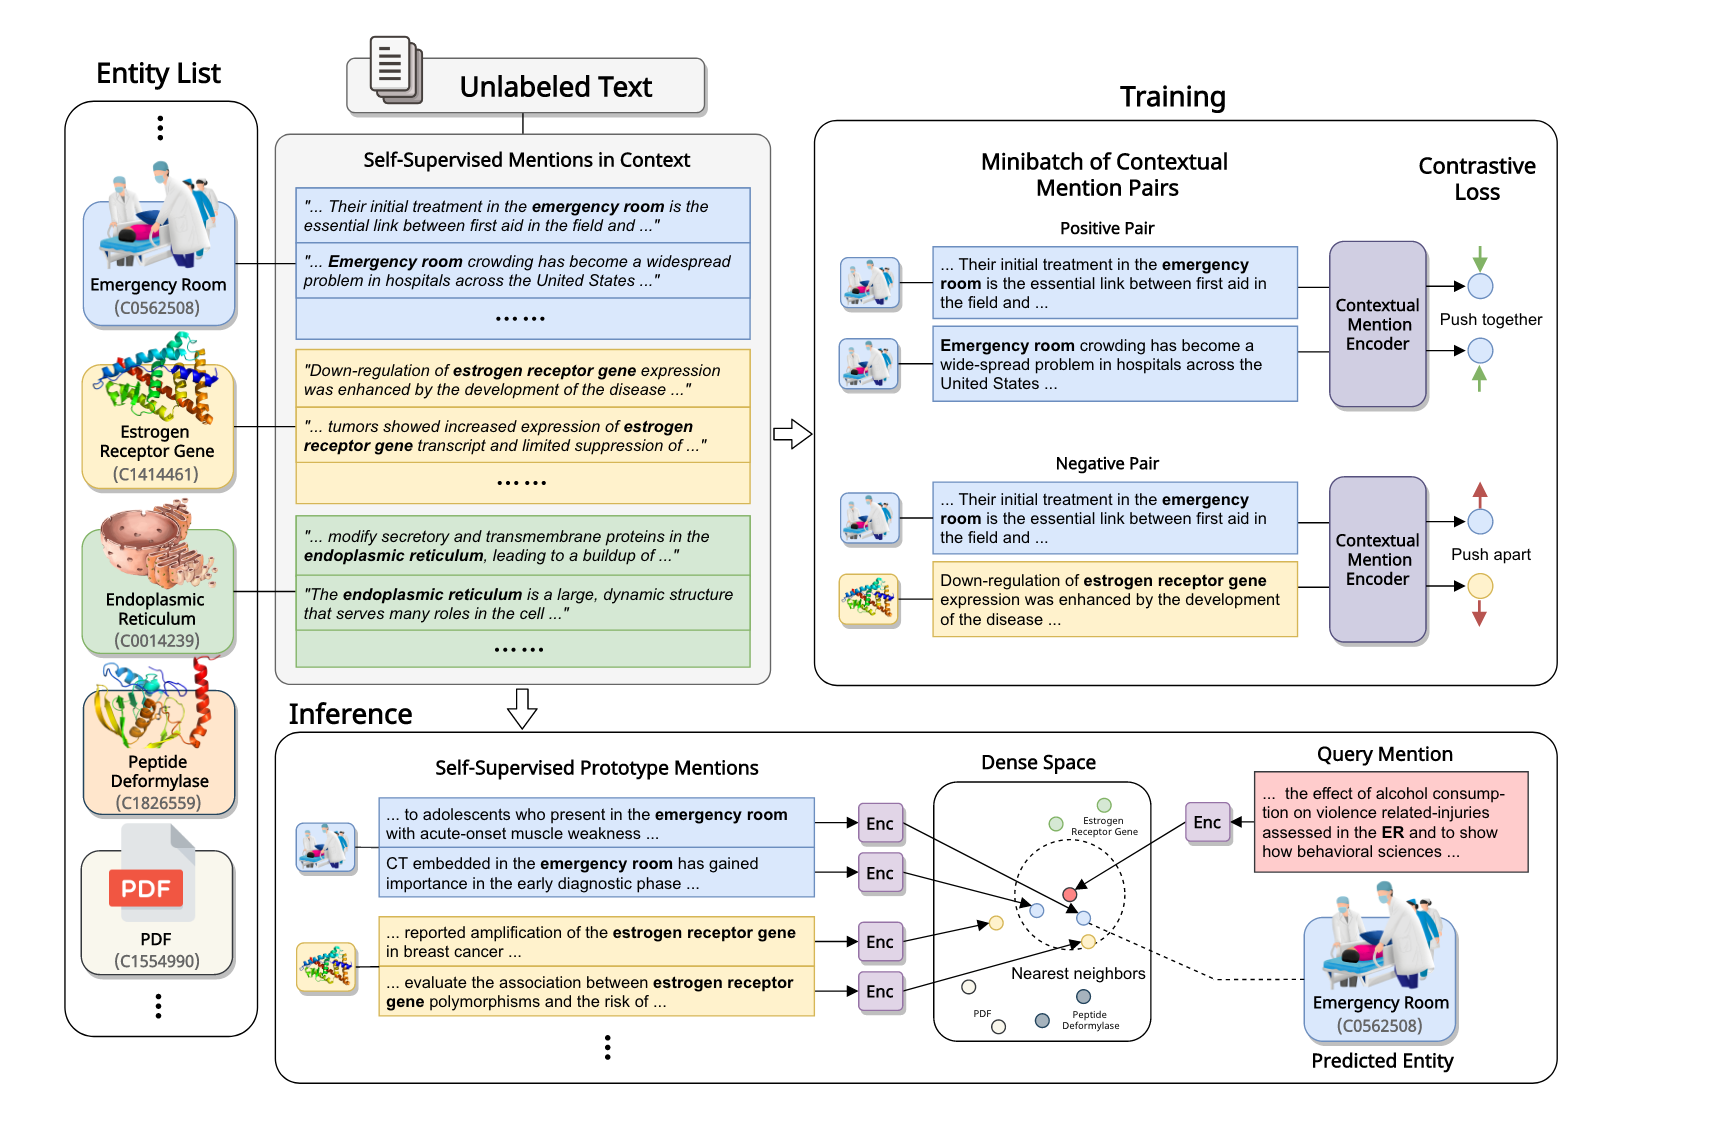
\includegraphics[scale=0.5]{images/KRISS-figure-1.png}
  \caption{From \cite{zhang_knowledge-rich_2022}}
  \label{fig:kriss}
\end{figure}

My baseline model will be \texttt{KRISSBERT} \cite{zhang_knowledge-rich_2022} (see Figure \ref{fig:kriss}). This self-supervised model is trained using the entire UMLS domain model. They compile a complete list of UMLS entity names into a trie, and use it to efficiently search text for entity mentions; they applied this string matching approach to PubMed abstracts and used it to generate 1.6 billion mention examples, each of which is uniquely linked to a UMLS entity concept identifier. They then use these mentions to train an entity encoder using contrastive loss \cite{oord_representation_2019}, initialized with PubMedBERT \cite{gu_domain-specific_2022}. They call the end result \texttt{KRISSBERT}, which is available for download on the Huggingface Hub (\url{microsoft/BiomedNLP-KRISSBERT-PubMed-UMLS-EL}). Inference is performed using a efficient and scalable form of nearest neighbor search \cite{johnson_billion-scale_2017}. They sample self-supervised mentions as prototypes for each entity and map the test mention to the most similar prototype.

Relation to datasets: The baseline \texttt{KRISSBERT} model is specifically designed to handle biomedical and clinical entity linking scenarios. My experiments will tie together this model with the datasets described above as follows:

\begin{itemize}
  \item I will first use PubMed and UMLS to re-implement the \texttt{KRISS} training algorithm and validate it against the MedMentions corpus, to see if I can reproduce the results for this dataset in \cite{zhang_knowledge-rich_2022}.
  \item I will then use the UMLS and the MIMIC-III notes table to generate a more clinically specific version of the model.
  \item I will use the ShARe and RadGraph datasets to test Hypotheses (3) and (4).
\end{itemize}

In relationship to the metrics described in the Metrics section, these will be used to measure performance on every version of clinical entity linking model that is generated to test the hypotheses.

% --------------------------------------------------------------------
\section{General reasoning}

The general approach is to augment self-supervised entity linking models with target specific domain information that can be used to improve entity linking performance, as measured by top-K accuracy and mean reciprocal rank. The baseline model is \texttt{KRISS}, which exhibits state of the art performance for self-supervised entity linking in the biomedical domain. Applying this approach to clinical notes, I believe we can do better by using clinically-focused resources, such as using ClinicalBERT \cite{huang_clinicalbert_2020} as the pre-trained model for mention embeddings, and filtering entities to smaller subsets of the UMLS for targeted use cases. Targeted datasets (such as radiology notes annotated with chest x-ray concepts) can be used to both fine-tune the mention embeddings model and improve inference by focusing just on concepts relevant to the use case.

% --------------------------------------------------------------------
\section{Summary of progress so far}

Completed steps:

\begin{enumerate}
  \item \checkmark Obtained access to the UMLS and have installed it on a local postgresql database on my macbook laptop.
  \item \checkmark Obtained the MedMentions dataset and written python code to parse it and convert it into a Pandas dataframe for ease of manipulation.
  \item \checkmark Obtained access to the MIMIC 3 note dataset, which required proper human subjects training. Physionet (the organization that distributes this dataset) also makes available a variety of other corpora, including RadGraph and ShaREe, which I have full access to through my Physionet account.
  \item \checkmark The \texttt{KRISSBERT} model and some test code are available through Huggingface (\url{huggingface.co/microsoft/BiomedNLP-KRISSBERT-PubMed-UMLS-EL}). I've cloned this code and executed it to generate prototype embeddings and run entity linking against the MedMentions corpus. Unfortunately, it does not appear that the authors have released the model training code for this project.
\end{enumerate}

Remaining steps:

\begin{enumerate}
  \item Implement the training algorithm as described in the paper
  \item Modify the entity mention generation algorithm to generate high-quality entity mentions, by imposing token length restrictions (and potentially other restrictions, based on analysis of generation errors).
  \item Evaluate performance of entity linker on target clinical domains (RadGraph, ShARe), using techniques described above for using a different base model, fine-tuning, pruning the entity set, etc.
\end{enumerate}

Concerns:

\begin{enumerate}
  \item My biggest concern is the ability to implement the \texttt{KRISS} training algorithm faithfully, based just on the details in the paper. I suspect this will be challenging and time-consuming.
  \item An easier task to envision is the entity pruning for targeted inference. Just implementing this would not require any changes to the \texttt{KRISSBERT} model, which I could simply use as is.
  \item Perhaps the easiest task (thanks to Huggingface) is fine-tuning \texttt{KRISSBERT} with target specfic data, such as all of MIMIC-III notes, or just the radiology notes, etc.
\end{enumerate}

% --------------------------------------------------------------------
\medskip
\printbibliography
\end{document}
